
\chapter{Introduction}
The quest to identify the origins of matter -- and consequently, the Universe itself -- has inspired us to delve deeper and deeper inside
the basic building blocks that constitute the atom. After the discovery of the atomic nucleus\cite{Rutherford:1911}, and subsequently individual
nucleons (protons and neutrons), these nucleons were considered as elementary particles until a further understanding of their building blocks
and constituent forces were reached. The developments in Quantum Chromodynamics shed light on another layer of matter lurking inside the
nucleons -- quarks and gluons -- and the binding force holding them together -- the strong interaction.

The leap from nucleons to quarks as the basic building blocks of matter is a considerable one and difficult to observe, as unlike nucleons,
quarks have not been identified to exist freely except in very special conditions involving extreme energy densities. These extreme
conditions "melt" the quark-gluon bonds in protons and neutrons, thereby enabling the deconfinement of quarks and gluons into a quasi-free state,
called the Quark-Gluon Plasma (QGP). The QGP state can only
be achieved through large energy densities, either by compressing the nucleonic matter or by deconfining quarks through thermal excitations.
The energy densities involved in the process of QGP's creation and its short lifetime render it a difficult, although not impossible, task to
reproduce this state for microscopic studies.

One way to achieve the necessary conditions for existence of QGP is by accelerating heavy ions close to the speed of light and colliding them,
thereby reaching the required energy density or temperature conditions. Although these conditions only exist for a minute period of time, and
the QGP would quickly cool down to produce ordinary hadronic matter before any direct measurements can be made, it is still possible to backtrack
the signs of its existence by studying the collective behaviour, generation and interaction of particles during the collision and other auxiliary
effects.

Particle accelerators for ion collider experiments like Brookhaven National Laboratory's Relativistic Heavy Ion Collider (RHIC)\cite{RHICqgp:2004},
CERN's Heavy Ion programme at Super Proton Synchrotron (SPS)\cite{SPSqgp:2000}, and the Large Hadron Collider (LHC)\cite{LHCqgp} at CERN have
dedicated experiments to create appropriate conditions suitable for probing into the existence of QGP. The LHC at CERN is the most powerful particle
accelerator so far, with collision energies reaching up to 13 TeV in Run 2. The ALICE (A Large Ion Collider Experiment)
detector\cite{ALICE} at LHC is designed to explore heavy-ion physics at extreme energy densities, focusing on lower interaction rate collisions
in order to achieve accurate particle identification, trajectory estimation, and energy calculations of daughter particles in a collision
such that precise assessments can be made about the collisionion epoch over a high range of multiplicities and momenta.

This work is dedicated to study a particular signature signifying the existence of QGP -- increased yield of strange and multi-strange particles
in ion collisions\cite{Bass:1999}. Commencing with an overview of theoretical and experimental studies on the subject, the topic of strangeness
production and its significance in strongly interacting matter and QGP is discussed. A brief description of the ALICE experiment with its subdetectors
is presented followed by the data collection and processing methodology. The analysis approach for the production of multi-strange baryons
$\Xi^{\pm}$ and $\Omega^{\pm}$ in p-Pb collisions at $\sqrt{s_{\textnormal{\sc nn}}}$ = 8.16 TeV during LHC's Run 2 data taking period are studied. Finally,
current results showing the raw $p_\textnormal{\sc t}$ spectra are presented.


\section{The Standard Model}
The Standard Model\cite{SM:2018,GriffithsSm:2008}, a culmination of numerous theories and discoveries towards an insight into the fundamental
structure of matter, aims to describe the fundamental particles and their interaction through the fundamental forces. All particle interactions
can be attributed to the four fundamental forces (Fig. \ref{fig:4forces}), or a combination thereof:
\begin{figure}[H]
  \centering
  \begin{subfigure}{.5\textwidth}
    \centering\captionsetup{width=.9\linewidth}%
    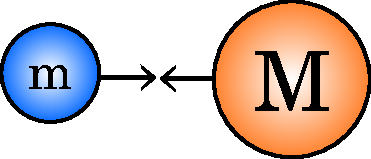
\includegraphics[width=.7\linewidth]{images/gravitational.pdf}
    \caption{Gravitation}
  \end{subfigure}%
  \begin{subfigure}{.5\textwidth}
    \centering\captionsetup{width=.9\linewidth}%
    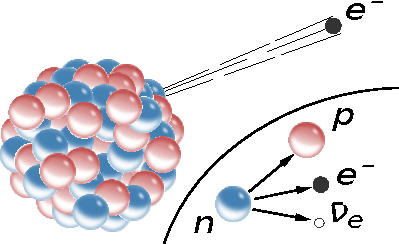
\includegraphics[width=.6\linewidth]{images/weak.pdf}
    \caption{Weak Interaction\cite{WeakForce:2021}}
  \end{subfigure}
  \begin{subfigure}{.5\textwidth}
    \centering\captionsetup{width=.9\linewidth}%
    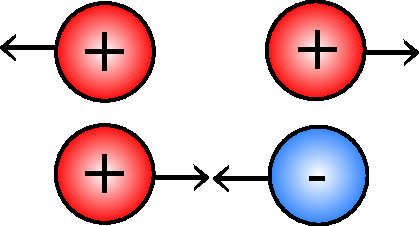
\includegraphics[width=.7\linewidth]{images/em.pdf}
    \caption{Electromagnetism}
  \end{subfigure}%
  \begin{subfigure}{.5\textwidth}
    \centering\captionsetup{width=.9\linewidth}%
    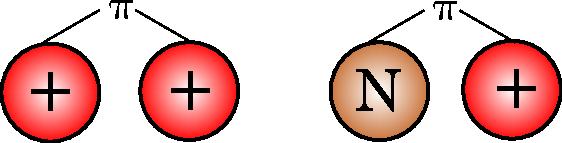
\includegraphics[width=.6\linewidth]{images/strong.pdf}
    \caption{Strong Interaction}
  \end{subfigure}
  \caption{The four fundamental forces}
  \label{fig:4forces}
\end{figure}

The Standard Model attempts to describe the particle physics phenomena through the unification of the fundamental forces at a sub-atomic level
(gravitational interaction, owing to its negligible effect on elementary particles, can be ignored at presently accessible energies)\cite{ShawMartin:2017}.
The inclusion of the the three fundamental forces in the model are described by their respective theoretical frameworks:
\begin{itemize}
  \item The electromagnetic interaction is described through Quantum Electrodynamics (QED)
  \item The strong interaction is described through Quantum Chromodynamics (QCD)
  \item The weak interaction can be described by electroweak unification, combining weak nuclear force with Quantum Electrodynamics
\end{itemize}

The strong interaction, aptly named being relatively the strongest of the four interactions, but with a short range, extends over the femtometer range
binding the quarks within the nucleons and the nucleons within the nucleus itself. It is also responsible for generating most of the mass of hadrons,
interacting between the color charges and described by Quantum Chromodynamics.

The electromagnetic interaction, whose electric and magnetic phenomena can be observed on a macroscopic scale, acts on all particles possessing an
electromagnetic charge. With an infinite range and second in strength after the strong interaction, the theoretical framework describing the EM
interaction is outlined by Quantum Electrodynamics.

The weak interaction, documented by the decay of unstable particles, is weaker in strength than the Strong and EM interactions, owing to heavier
force-carrier particles resposible for the interaction (\textsl{W} and \textsl{Z} bosons). Energies in excess of mass of these bosons render EM and
weak interactions with a comparative strength, and clubbed together, they are explained by the unified theory of electroweak interactions. The theory
also incorporates the Higgs field and the Higgs mechanism, reponsible for mass generation in elementary particles.

The gravitational interaction, relatively being the weakest of the four forces, has an infinite range acting over all massive particles and can
be described by Einstein's general theory of relativity. Due to its infinitesimal impact on the sub-atomic scale when compared to the other three
forces, it is not a part of the Standard Model. However, on a macroscopic scale, gravitational interaction holds a much more
significant position, prevailing over the short-ranged strong and weak nuclear forces, while most electromagnetic interactions are screened due
to electrically neutral nature of atoms.

The Standard Model also sheds light on the origin of these forces, especially relevant at short distances when quantum effects become significant. This
assertion is based on particle interaction through an exchange of force-carrier particles classified as gauge bosons, a subset of bosons - a broader
class of particles described further in this section. Each fundamental force is
described by its corresponding gauge boson responsible for discrete energy transfer. Table \ref{tab:GriffithsSmTable} lists the four fundamental
forces and their theoretical frameworks, their comparative strengths and corresponding gauge bosons.

\begin{table}
  \centering
  \begin{tabular}{lrll}
    Force           & Strength   & Theory           & Mediator\tabularnewline
    \hline
    Strong          & 10         & Chromodynamics   & Gluon\tabularnewline
    Electromagnetic & 10$^{-2}$  & Electrodynamics  & Photon\tabularnewline
    Weak            & 10$^{-13}$ & Flavourdynamics  & \textsl{W} and \textsl{Z}\tabularnewline
    Gravitational   & 10$^{-42}$ & Geometrodynamics & Graviton\tabularnewline
    \hline
  \end{tabular}
  \caption{The four fundamental forces\cite{GriffithsSmTable:2008}}
  \label{tab:GriffithsSmTable}
\end{table}

Primarily, the Standard Model classifies elementary particles into two main classes: \textit{bosons} and \textit{fermions}. Fermions, regarded as the
building blocks of matter, exist in 24 variants including their particle and anti-particle counterparts. The elementary fermions are subdivided
into quarks and leptons, each with a unique mass, ${\textstyle \frac{1}{2}}$ spin value (thus obeying the Pauli exclusion principle), and an
electrical charge (except for the electrically neutral neutrinos). The antiparticle counterparts carry over the same mass but opposite quantum
numbers (electrical charge, lepton number, etc.). Although the fermions exhibit the same electric charge and similar interaction capabilities for the
weak and strong nuclear forces across the three generations, the primary difference noted among the generations lies in their increasing trend of
average mass (Fig. \ref{fig:SmElementaryParticles}) depending on their coupling with the Higgs field.
Fermions obey the Fermi-Dirac statistics, and combine together to form composite particles such as hadrons, nuclei and atoms, which can be bosonic or fermionic in their nature depending
on the constituents involved.


\begin{figure}[H]
  \centering
  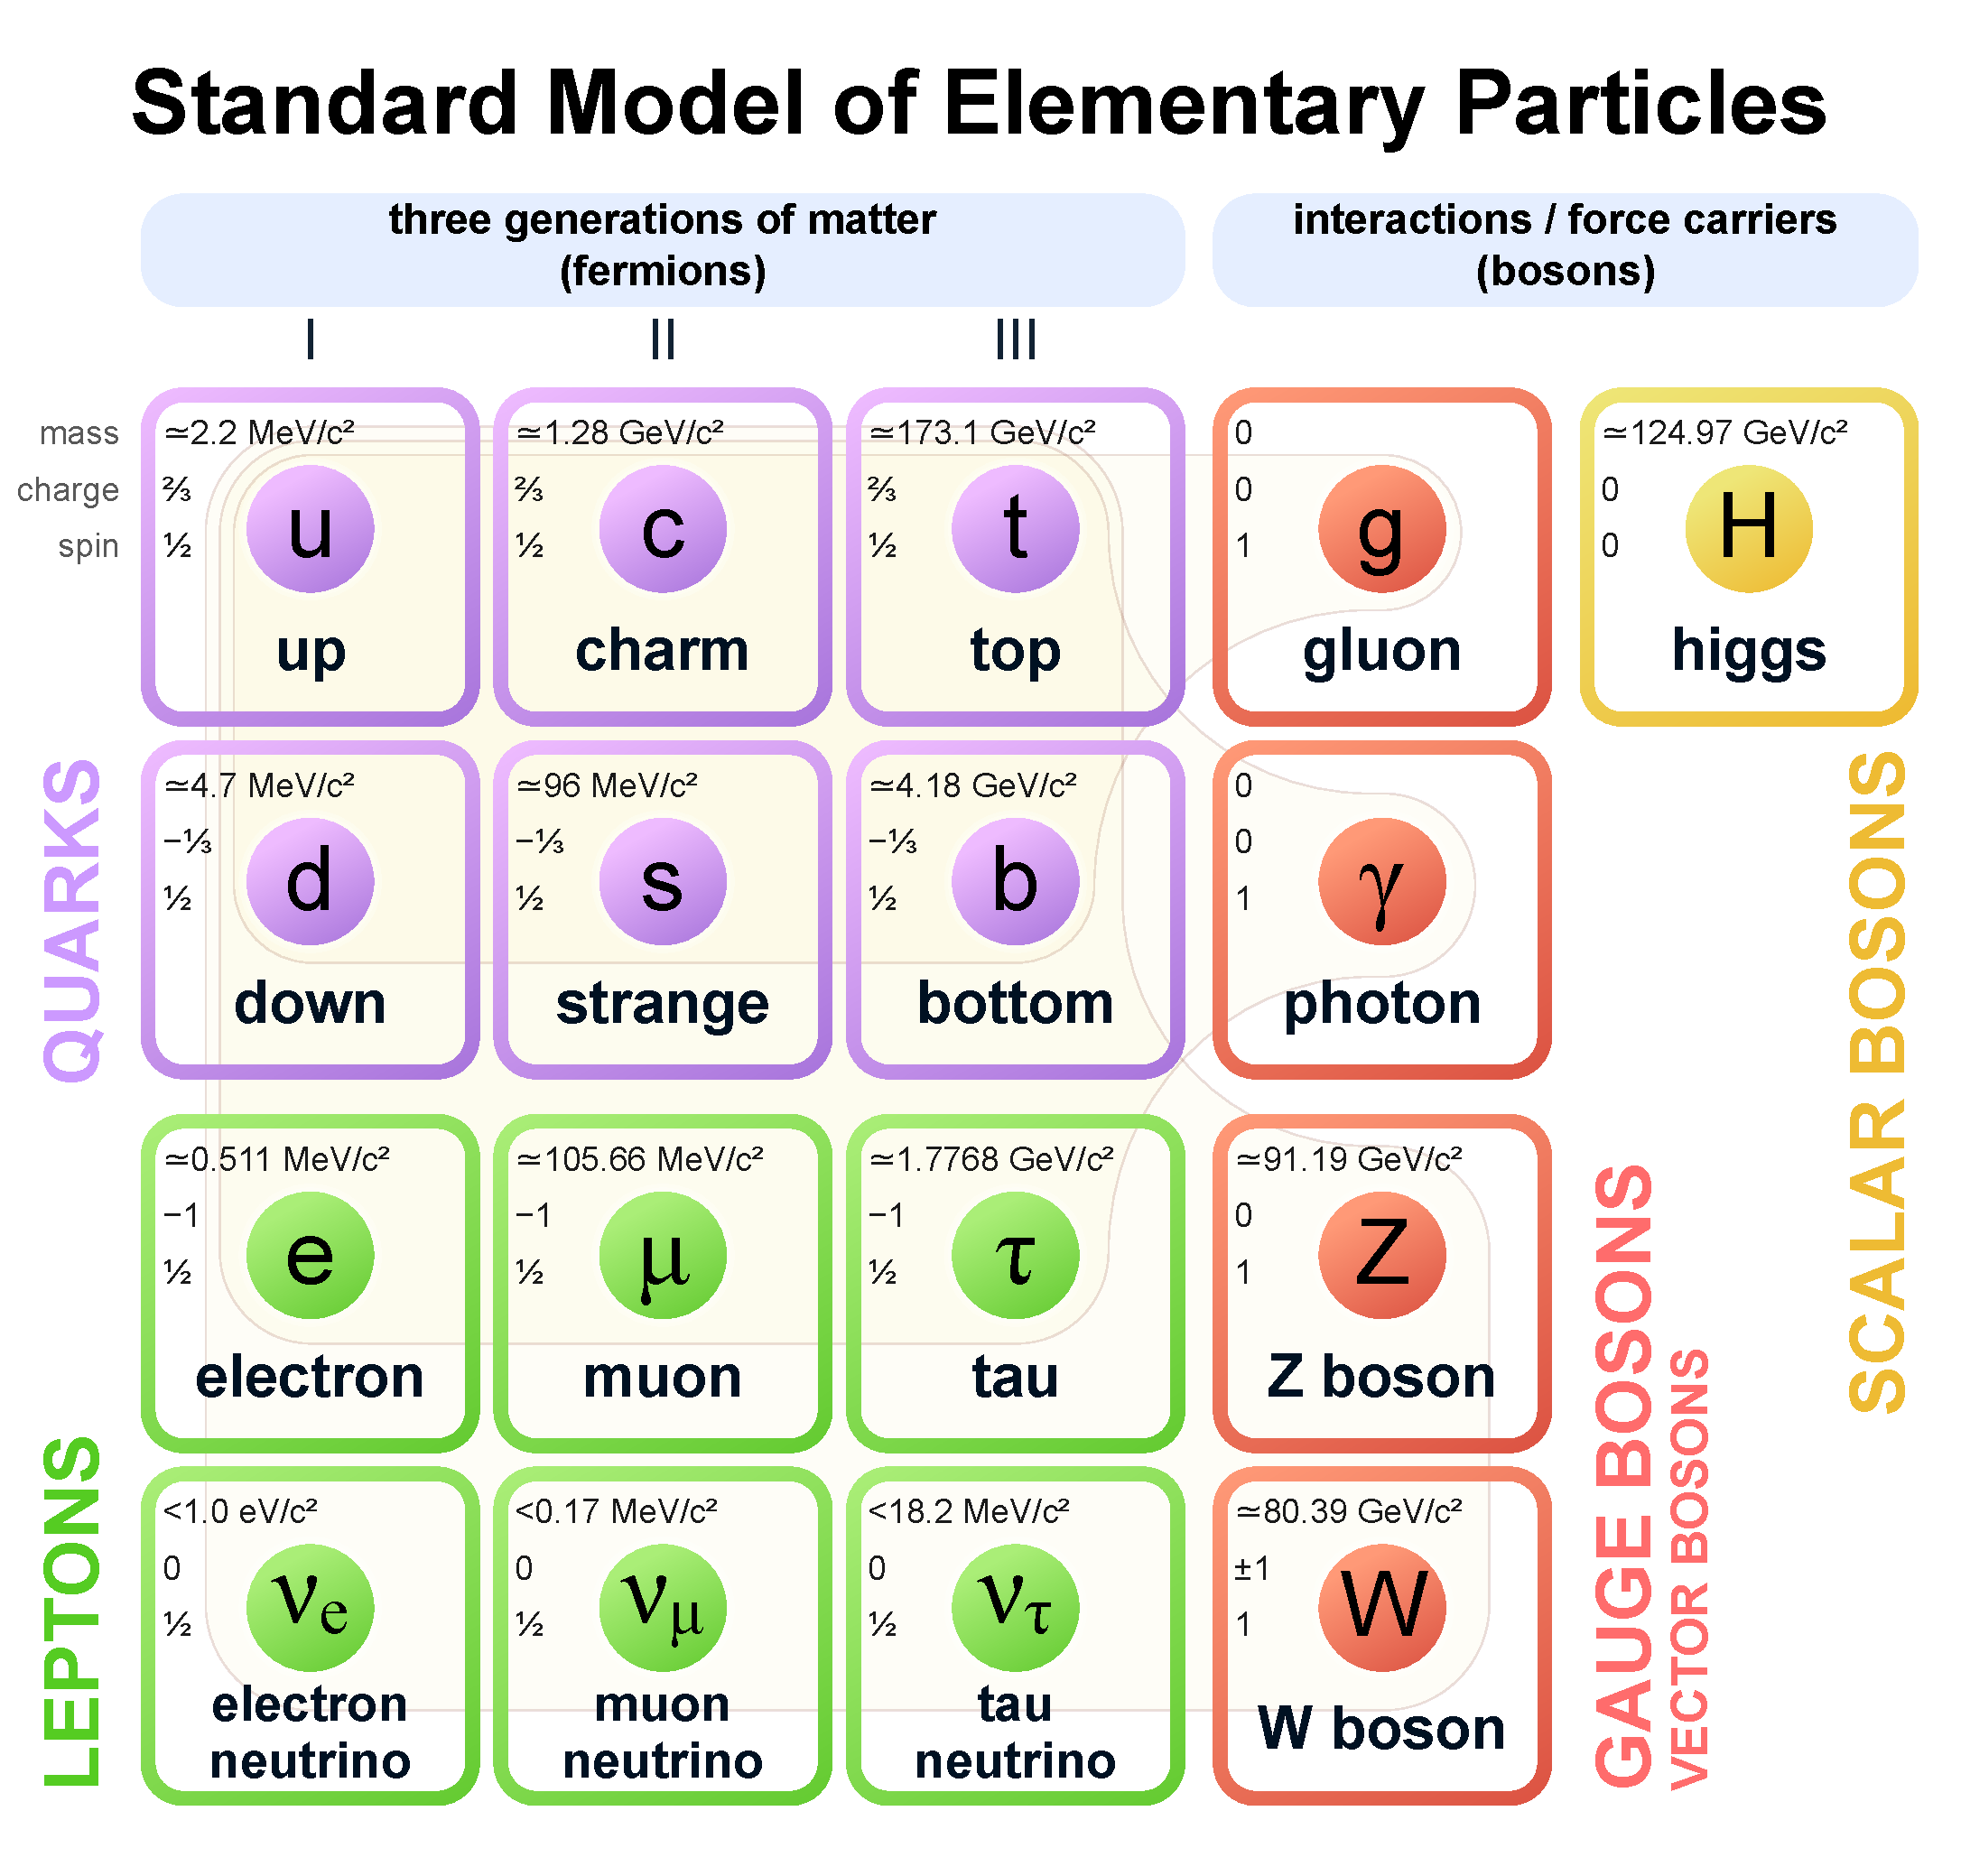
\includegraphics[width=0.9\linewidth]{images/SmElementaryParticles.pdf}
  \caption{Standard Model of Elementary Particles\cite{SmElementaryParticles}. Corresponding antiparticles exist for all listed particles,
    except for $g, \gamma, Z^{0}$ and $H$ (which are their own antiparticles).}
  \label{fig:SmElementaryParticles}
\end{figure}


Bosons, on the other hand, have integer spin values (spin-0 or spin-1) which exempts them from the Pauli exclusion principle. Currently, the Standard
Model encapsulates five different bosons, out of which four of them are known as gauge bosons (spin-1) which act as the force-carriers for the
aforementioned three fundamental forces. The gluon (\textit{g}) acts as the mediator for the strong interaction, photon (\textit{$\gamma$}) for the
electromagnetic interaction and the \textit{W$^{\pm}$} and \textit{Z$^{0}$} bosons act as mediators for the weak interaction. The fifth boson, scalar
in nature with a spin-0 value, is a recently discovered member to the Standard Model. This particle, known as the Higgs boson, is deemed to be
responsible for assigning mass to particles. Bosons follow the Bose-Einstein statistics for the formation of composite particles.

\begin{figure}
  \centering
  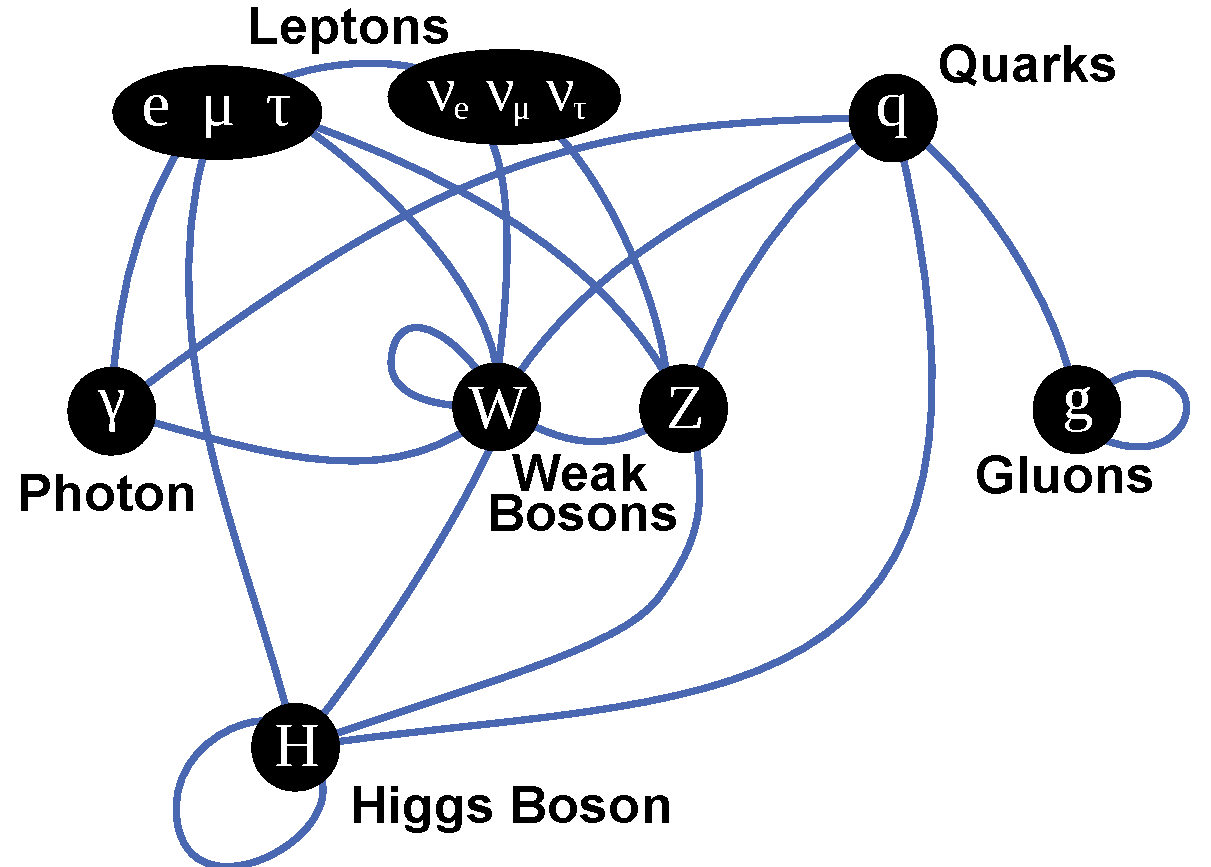
\includegraphics[width=0.75\linewidth]{images/ElementaryParticleInteractions.pdf}
  \caption{Interactions between Elementary Particles\cite{ElementaryParticleInteractions}}
  \label{fig:ElementaryParticleInteractions}
\end{figure}


The interactions among elementary particles and their combinations are outlined in Fig. \ref{fig:ElementaryParticleInteractions}, with closed curves
depicting interactions within the
group. The Higgs boson interacts with itself and all massive particles, the quarks interact via strong interaction with all bosons and particles
possessing a 'colour' charge. Gluons exhibit quark-gluon interaction alongwith self-interaction, which is discussed further in the next sections.

\section{Quantum Chromodynamics}
Quantum Chromodynamics (abbreviated as 'QCD') is a theoretical framework that aims to explain the mechanics of the strong interaction, alongwith the
fundamentals pertaining to the nature and conduct of quarks and gluons (collectively known as partons). Apart from the aforementioned attributes of
unique mass and an electrical charge, QCD defines partons to possess an additional quantum number known as 'colour' charge. The concept of colour
charge was first put forward by Oscar W. Greenberg\cite{OWG:1964}, M. Han and Y. Nambu\cite{HanNambu:1965}, justifying the coexistence of quarks in
identical quantum states bound in hadrons without violating Pauli's
exclusion principle. As an example, the discovery of delta baryon --  $\Delta^{++}$ (u,u,u) consisting of three up quarks with parallel spin could
be validated.

The colour quantum number exists in three equivalent states, dubbed as red, green and blue. Much like its electromagnetic counterpart, each colour
charge has its corresponding antiparticle colour state (Fig. \ref{fig:colorCharge}); and similar to the photon's coupling to the electromagnetic
charge in QED, the gluon couples to the colour charge in QCD. However, unlike the photon, the gluon carries the charge of the colour it mediates,
thereby enabling self-interaction while also participating in the strong interaction. Contrary to quarks which carry a single colour charge, gluons
carry both the colour and anti-colour charge. The gluon-gluon and gluon-quark interactions maintain the conservation of colour charge. The colour
charge is also confined, i.e. the colour charged particles cannot be isolated and must remain in conjunction as colourless hadrons (also stated as
colour-singlets) below the Hagedorn temperature ($\sim10^{12} K)$. This phenomenon is termed as colour confinement\cite{FlorkowskiColour:2010} and is
responsible for the absence of free quarks and gluons.

\begin{figure}[H]
  \centering
  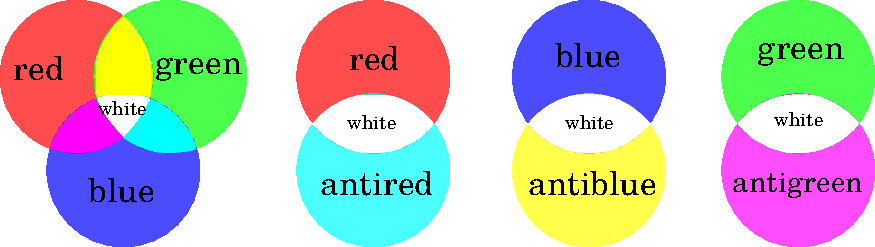
\includegraphics[width=0.7\linewidth]{images/colorCharge.pdf}

  % \textit{Baryons\hspace{6.5cm}Mesons}
  \caption{An illustration depicting the colour charges and their combinations. Baryons are composed of red, green and blue colour charges (left),
    while a singular pair of colour-anticolour combination forms a meson, as shown in the last three diagrams.}
  \label{fig:colorCharge}
\end{figure}

The gluon self-interaction causes anti-screening due to quantum fluctuations, and the probability for this effect increases with distance between
quarks. This effect gives rise to a phenomenon known as asymptotic freedom\cite{Gross:1973,Politzer:1973}, indicating that larger distances between interacting
quarks lead to increased strength of the strong interaction. The strength of the strong interaction can be measured by its running coupling constant
$\alpha_{s}$, which can be defined as follows\cite{FlorkowskiCoupling:2010}:

\medskip
\begin{equation}
  \alpha_{s}(Q^{2})=\frac{16\pi^{2}}{(11 - \frac{2}{3}N_{f})ln(\frac{Q^{2}}{\Lambda_\textnormal{\sc qcd}^{2}})} \hspace{0.15cm} \xrightarrow{Q^{2}\to\infty} 0,
  \label{eq:CouplingQCD}
\end{equation}
\smallskip

where Q is the Lorentz invariant generalisation of momentum transfer, $N_{f}$ is the number of included quark flavours that can partake in the
screening loop and $\Lambda_\textnormal{\sc qcd}$ is the QCD scale parameter determined either experimentally or from lattice QCD calculations such that the
coupling constant is calibrated at mass of $Z^{0}$ boson ($\Lambda_\textnormal{\sc qcd} \approx 200$ MeV). From the experimental results (Fig. \ref{fig:CouplingQCD}),
the dependence of $\alpha_{s}$ on $Q$ can be confirmed. At short distances, the
coupling constant vanishes, implying that parton interactions are negligible in the limit of very high temperatures\cite{Gross:1973,Politzer:1973}.
This occurrence points to the creation of a virtually non-interacting QGP at extreme temperatures\cite{Collins:1975,Cabibbo:1975}.

\begin{figure}[H]
  \centering
  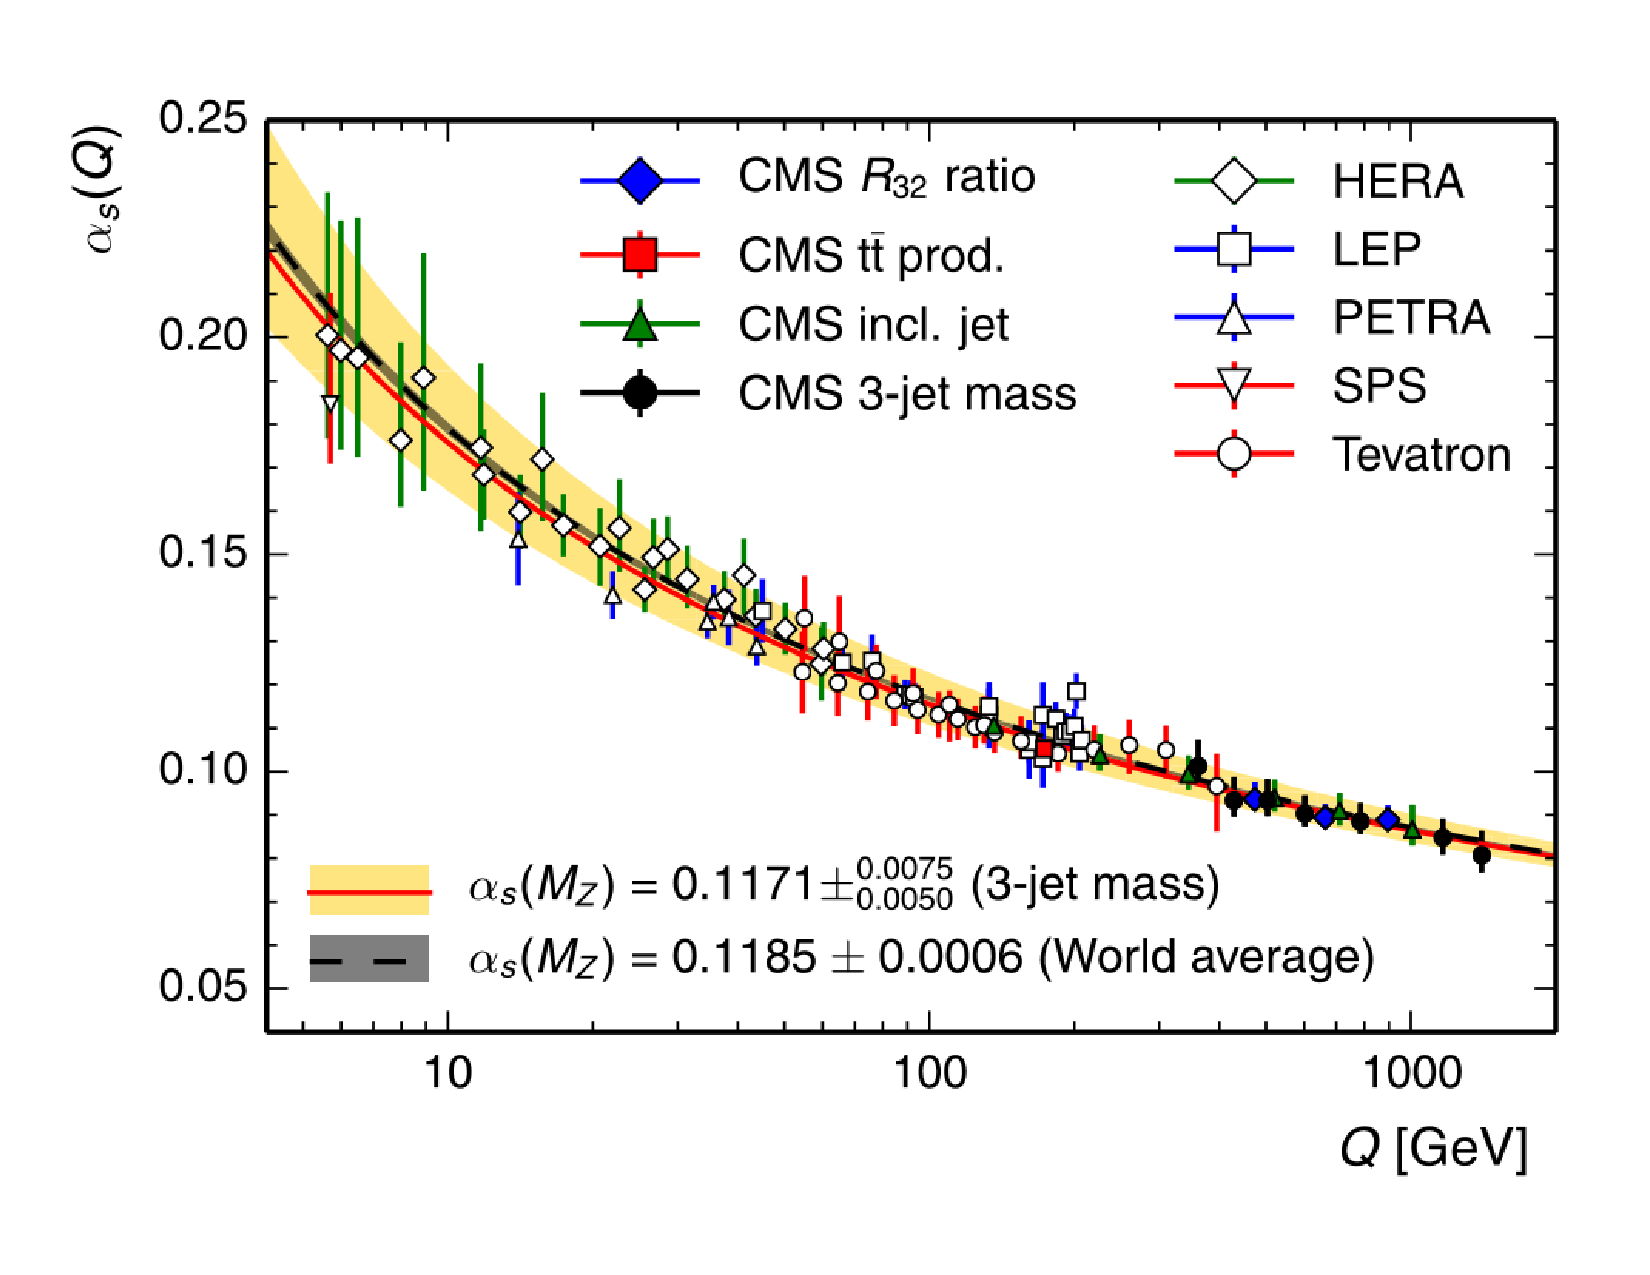
\includegraphics[width=0.7\linewidth]{images/CouplingQCD.pdf}
  \caption{Comparison of $\alpha_{s}$ evolution as measured by different experiments\cite{CouplingQCD:2015}.}
  \label{fig:CouplingQCD}
\end{figure}

\section{Quark-Gluon Plasma}

As stated earlier, the phenomenon of colour confinement points to a bound state of quarks and gluons within hadrons in ordinary circumstances.
However, the existence of a phase consisting of deconfined quarks and gluons achieved by high temperatures and/or significant net baryon densities
has been hypothesised early on and presumed to exist in neutron stars and the early universe, shortly after the Planck epoch\cite{PlanckEpoch} according to the Big Bang
theory\cite{bigBang}.
Attempts to recreate this primordial liquid have been carried out by various particle accelerators and collider experiments making use of
immense pressure values to 'merge' the hadrons together and creating high enough temperatures to excite quarks out of their bound state in hadrons.
The extreme temperature ($\sim 1.97\times10^{12}$ K) and particle density should result in the merging of confined partons to an incredibly hot,
superdense quark-gluon 'soup' (Fig.\ref{fig:qgp}), where free quarks could exist. Particle collisions at the Large Hadron Collider are believed
to exhibit conditions sufficient for the creation of this new state of matter.

\begin{figure}[H]
  \centering
  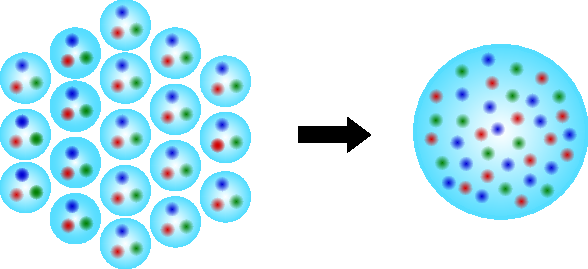
\includegraphics[width=0.7\linewidth]{images/qgp.pdf}
  \caption{An illustration depicting isolated hadrons merging into a quark-gluon plasma.}
  \label{fig:qgp}
\end{figure}

Although named as a plasma based on the assumption that the QGP would be exhibiting properties akin to an ultrahot gas of charged particles, the
quark 'soup', in essence, behaves as a nearly perfect Fermi liquid: the strongly coupled QGP (sQGP)\cite{HeinzRHIC:2005}. Models based on relativistic
hydrodynamics at the LHC and RHIC have been able to effectively describe the fluid-like characteristics and related observables like elliptic flow,
radial expansion and higher order flow harmonics.

The grand canonical ensemble characterises nuclear matter in thermodynamic equilibrium with respect to temperature $T$, volume $V$, and the
baryo-chemical potential $\mu_\textnormal{\sc b}$. Here, $\mu_\textnormal{\sc b}$ is the chemical potential of the conserved baryon number. Figure \ref{fig:QcdPhaseDiagram}
depicts a schematic representation of the phase diagram of nuclear matter in the $\mu_\textnormal{\sc b}, T$ plane. Nuclear matter, ordinarily, exists at
$T\approx0$ and $\mu_\textnormal{\sc b}\approx1$ GeV. The phase boundary ending in a critical end-point differentiates the hadron resonance gas phase from the
quark-gluon plasma. For a critical point $E$ on the diagram, lattice QCD approach determines $T_\textnormal{\sc e}\approx160$ MeV and $\mu_\textnormal{\sc e}\approx725$ MeV\cite{Fodor:2002}.
At minimal $\mu_\textnormal{\sc b}$ values,
the critical temperature for transition's cross-over is ($T_\textnormal{\sc c}\approx170$ MeV). On the other hand, at low values of temperature but baryon density
exceeding a few times of nuclear matter density, a deconfined color superconducting phase is predicted, perhaps along with other phases\cite{Fukushima:2013}.

According to recent lattice calculations, a slightly lower transition temperature ($T_\textnormal{\sc c}\approx155$ MeV) is forecasted\cite{Bazavov:2012, Bhattacharya:2014},
which agrees well with the statistical hadronisation model's chemical freeze-out temperature\cite{Andronic:2009}.

\begin{figure}
  \centering
  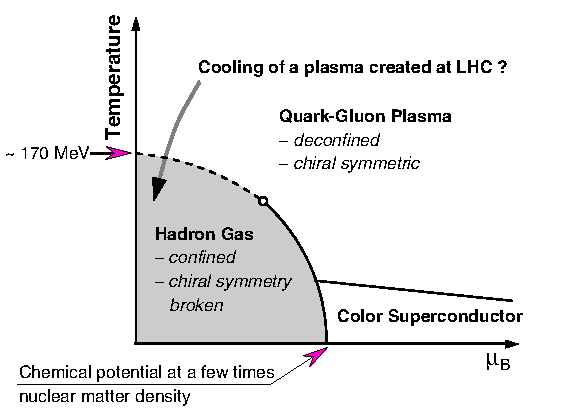
\includegraphics[width=0.8\linewidth]{images/QcdPhaseDiagram.pdf}
  \caption{\small The phase diagram of QCD: solid lines indicate first-order transitions, dashed lines indicating possible continuous rapid
    crossover transition\cite{Carminati:2004}.}
  \label{fig:QcdPhaseDiagram}
\end{figure}


The QGP state, by itself, is quite unstable owing to the extreme conditions required for its creation and sustainability, hence it exists for a
microscopic amount of time before cooling down and re-confining back to the hadron state. At LHC energies, the expected lifetime of QGP is
judged to be 4 to 6 fm/c\cite{Sahoo:2010}, hence any observation for its formation are required to be probed in this interval or at the
earliest collision moment so as to avoid any subsequent hadronisation. This presents a challenge to make direct observations for QGP's existence
owing to its limited lifetime to verify its creation on a macroscopic scale.
Therefore, its existence and effects must be studied indirectly by observing the auxiliary phenomena as signatures of QGP\cite{Bass:1999}$\colon$
\begin{enumerate}
  \item Production of direct (thermal) photons and thermal dileptons
  \item Suppression of J/$\psi$ and $\psi^{\prime}$ particle production
  \item Increased yield of strange and multi-strange hadrons
  \item Jet Quenching
  \item Suppression of the production of hadrons with high transverse momentum
  \item Collective (Elliptic, directed, and transverse) flow of baryons and mesons
  \item Increased baryon production at mean transverse momentum
  \item Change in the mass and lifetime of vector mesons
\end{enumerate}

In this thesis, the increased yield of multi-strange baryons in high energy collisions is studied. The production of multi-strange cascade baryons
such as $\Xi^{\pm}$ and $\Omega^{\pm}$ in p-Pb collisions at LHC energies $\sqrt{s_{\textnormal{\sc nn}}}$ = 8.16 TeV in the ALICE detector are presented. An overview
comprising of the theoretical and experimental advancements in the realm accompanied by the importance of strangeness studies in strongly interacting
matter and as a signature of the quark-gluon plasma is discussed. Analysis details, consisting of the detector layout and important sub-detectors
pertaining to the data collection and particle information necessary for analysis, data sample, processing, analysis and filtering
to obtain good candidates for reconstruction, subsequent analysis methods and follow up tasks are explained. Summing up with the current status of
the analysis and raw $p_{\textnormal{\sc t}}$ spectra results, the final goals and outlook is presented.



